\documentclass{beamer}

\usepackage{amsthm, amsfonts, amsmath, amssymb} % Pacote para a definicao dos ambientes matematicos
\usepackage[brazilian]{babel}
\usepackage[utf8]{inputenc}
\usepackage[mathscr]{eucal}
\usepackage{tikz}
\usetikzlibrary{quotes, angles, intersections}
\newcommand{\R}{\mathbb{R}}
\newcommand{\D}{\mathscr{D}}
\newcommand{\Pp}{\mathscr{P}}
\newcommand{\bigO}{\mathscr{O}}
\newcommand{\Cc}{\mathscr{C}}
\newcommand{\E}{\mathscr{E}}
\newcommand{\F}{\mathscr{F}}
\newcommand{\Ww}{\mathscr{W}}
\newcommand{\Rr}{\mathscr{R}}
\newcommand{\norm}[2][2]{\left\lVert#2\right\rVert_{#1}}

\author{Danilo Tedeschi\\Dra. Marina Andretta}
\title{Algorithms for Planar Maximum Covering Location by Ellipses Problems}
\institute{Universidade de São Paulo}
\date{25 de Outubro de 2019}


\begin{document}
	
	\begin{frame}[t,plain]
		\titlepage
		
		\footnotesize This research has been funded by Cordenação de Aperfeiçoamento de Pessoal de Nível Superior (CAPES). This is part of a Master's research project on the problem: \textit{Planar Maximal Covering by Ellipses with Rotation}.
	\end{frame}
	
\begin{frame}{Introduction}
	
	Two versions: 
	\begin{itemize}
		\item Planar Maximum Covering Location by Ellipses Problem (MCE) \cite{canbolat};
		\item Planar Maximum Covering Location by Ellipses with Rotation Problem (MCER) \cite{andreta}.
	\end{itemize}
\end{frame}

\begin{frame}{Introduction}{Ellipse}
	The shape of an ellipse is given by its major-axis and minor-axis, $(a, b) \in \mathbb{R}^2$, with $a > b > 0$.
	
	\begin{figure}[H]
		\centering
		
		%\caption{The ellipse as a parametric curve.}
		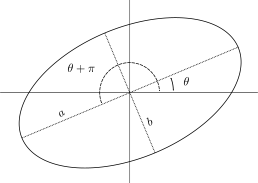
\includegraphics[scale=.3]{../tex/figures/rotated_ellipse.pdf}
		\label{fig:ellipse_params}
		\caption{An ellipse with shape parameters $a$ and $b$.}
	\end{figure}
	
\end{frame}

\begin{frame}{MCE}
	\begin{block}{Definition}
		Demand set $\Pp=\{p_1, \dots, p_n\}$;\\
		Weights $\Ww = \{w_1, \dots, w_n\}$;\\
		Shape parameters $\Rr = \{(a_1, b_1), \dots, (a_m, b_m)\}$, $a_j > b_j > 0$.\\
		Set of functions $\E = \{E_1, \dots, E_m\}$, $E_j(q_j)$ is the $j$-th ellipse's coverage region.
	\end{block}
\end{frame}

\begin{frame}[allowframebreaks]
	\frametitle{References}
	\bibliographystyle{amsalpha}
	\bibliography{../references.bib}
\end{frame}
	
\end{document}